\chapter{Planos de Ingeniería del Proyecto}

Los planos del proyecto han sido vectorizados en formato DXF compatible con AutoCAD/QCAD y exportados en PDF/PNG de alta definición para su consulta impresa. A continuación se presentan las vistas esquemáticas oficiales del proyecto:

\section{Plano IE-01: Diagrama Unifilar General TGD}
Muestra la acometida desde la Red Pública, transformador $T_1$ de $100\text{ kVA}$, barra $R-S-T-N$, ITM General de 100A, TGD, sub-tableros TF1/TI1, banco de condensadores C7 de $15\text{ kVAr}$ y los 7 circuitos derivados con conductores N2XH y protecciones.

\begin{figure}[H]
  \centering
  \IfFileExists{figuras/industrial_unifilar.png}{%
    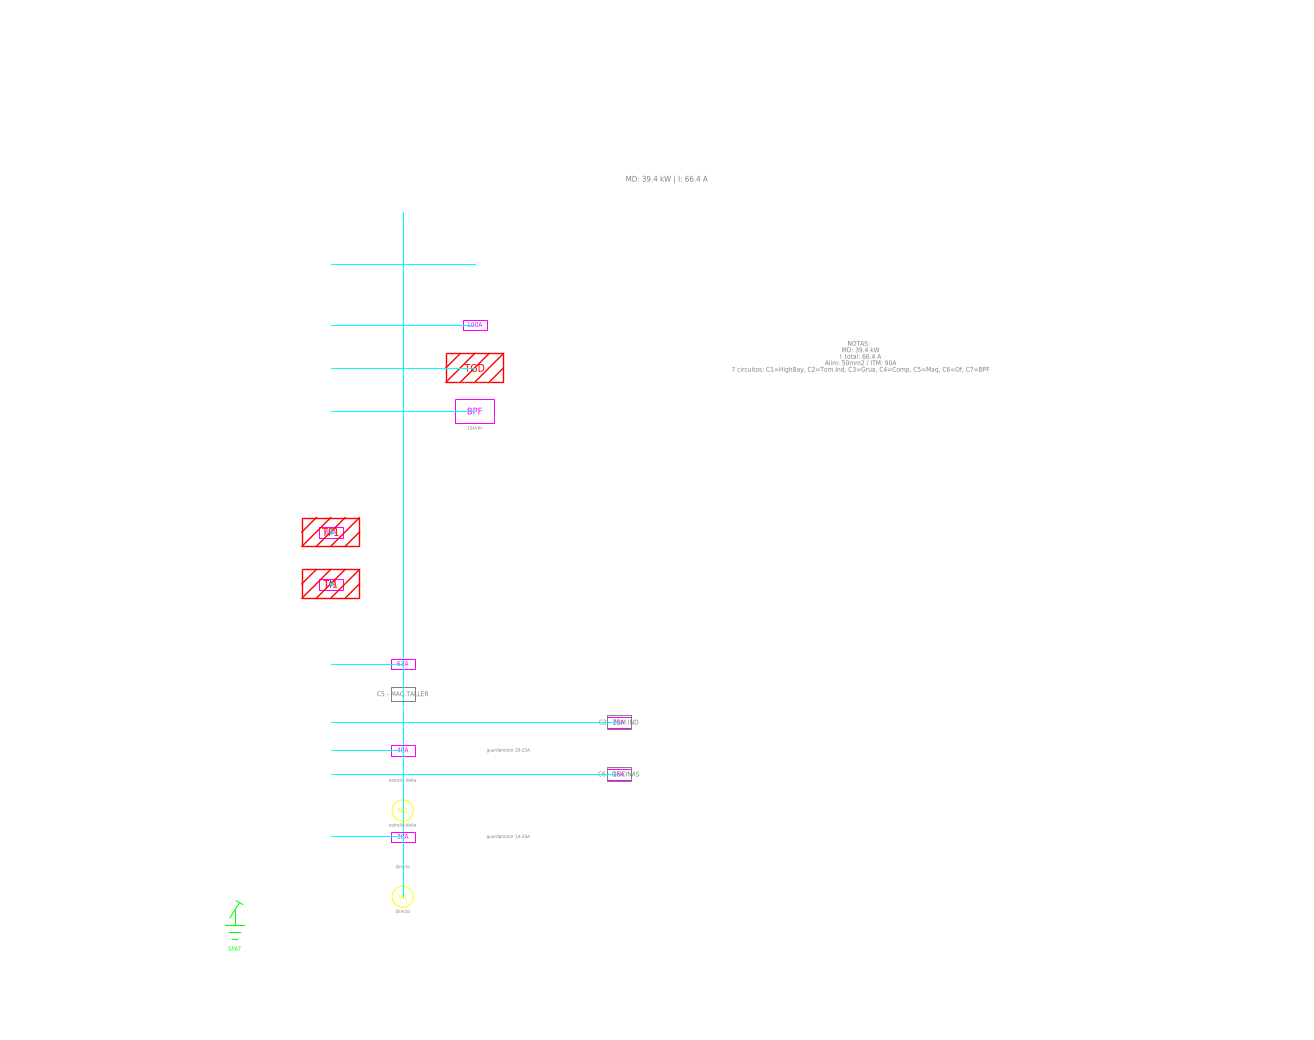
\includegraphics[width=0.95\textwidth]{figuras/industrial_unifilar.png}%
  }{%
    \textbf{[Plano 01: industrial\_unifilar.pdf / dxf]}%
  }
  \caption{Plano IE-01: Diagrama Unifilar General - TGD Nave Industrial 20x40m.}
  \label{fig:unifilar_ch}
\end{figure}

\clearpage
\section{Plano IE-02: Distribución en Planta y Malla SPAT}
Muestra las 4 zonas operativas (Producción, Almacén, Oficinas y SS.HH.), la ubicación simétrica de las 20 campanas LED High-Bay a $7\text{ m}$, tomas Stecker 380V, motores M1/M2 y la **Malla SPAT perimetral de 6 varillas enterradas a $0.80\text{ m}$**.

\begin{figure}[H]
  \centering
  \IfFileExists{figuras/industrial_distribucion.png}{%
    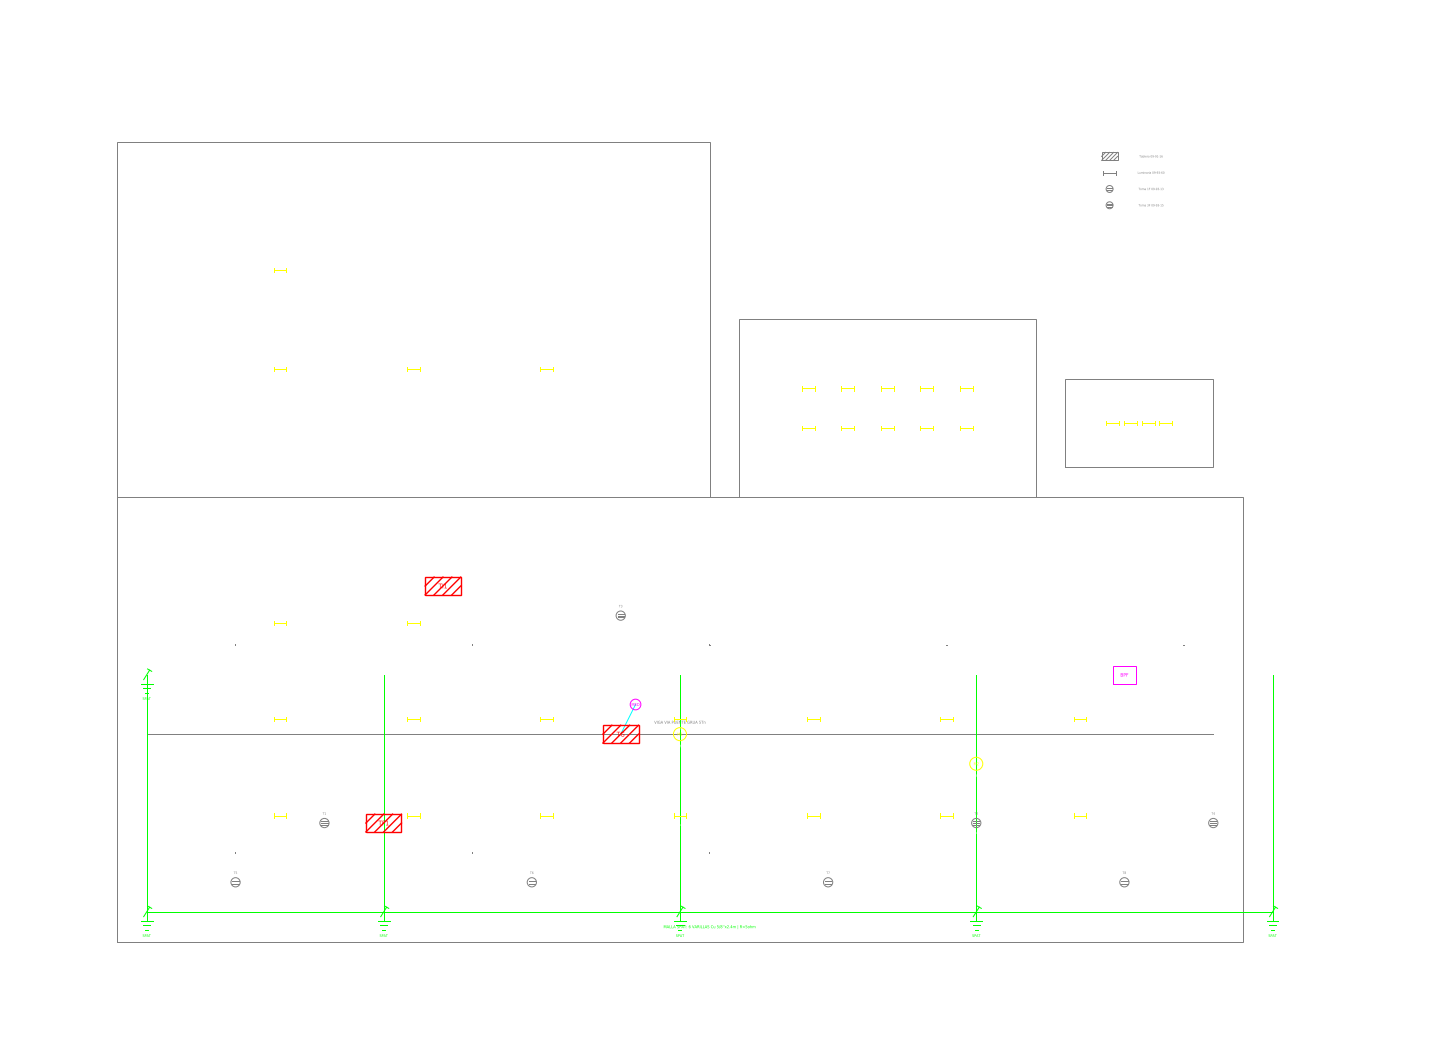
\includegraphics[width=0.95\textwidth]{figuras/industrial_distribucion.png}%
  }{%
    \textbf{[Plano 02: industrial\_distribucion.pdf / dxf]}%
  }
  \caption{Plano IE-02: Distribución en Planta y Malla SPAT Perimetral ($R < 5.0\:\Omega$).}
  \label{fig:distribucion_ch}
\end{figure}

\clearpage
\section{Plano IE-03: Diagrama de Fuerza y Centro de Control de Motores (MCC)}
Detalla las protecciones magnetotérmicas ajustables (guardamotores) y esquemas de arranque directo DOL para el Puente Grúa M1 (10HP) y Estrella-Delta para el Compresor M2 (15HP) y Maquinaria de Taller C5 ($25\text{ kW}$).

\begin{figure}[H]
  \centering
  \IfFileExists{figuras/industrial_fuerza.png}{%
    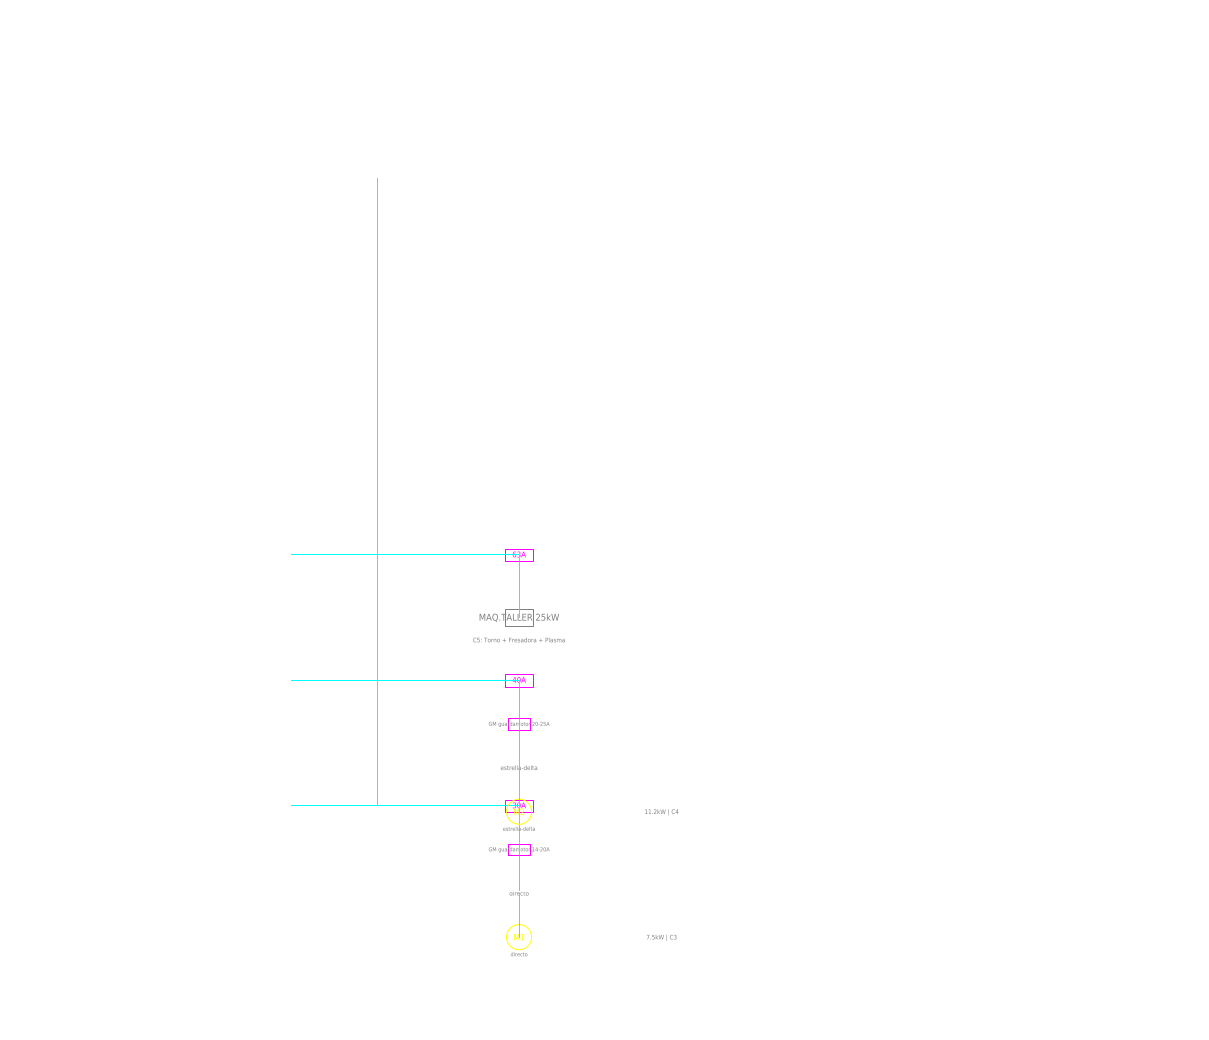
\includegraphics[width=0.95\textwidth]{figuras/industrial_fuerza.png}%
  }{%
    \textbf{[Plano 03: industrial\_fuerza.pdf / dxf]}%
  }
  \caption{Plano IE-03: Diagrama de Fuerza MCC (Guardamotores y Arranque E-D).}
  \label{fig:fuerza_ch}
\end{figure}
